\documentclass[12pt]{kiarticle} 
\graphicspath{{pic/}}
\DeclareGraphicsExtensions{.pdf,.png,.jpg,.eps}
%%%
\pagestyle{fancy}
\fancyhf{}
%\renewcommand{\headrulewidth}{ 0.1mm }
\renewcommand{\footrulewidth}{ .0em }
\fancyfoot[C]{\texttt{\textemdash~\thepage~\textemdash}}
\fancyhead[L]{Лабораторная работа № 3.24 \hfil}
\fancyhead[R]{\hfil Иванов Кирилл, 625 группа }
\usepackage{multirow} % Слияние строк в таблице
\newcommand
{\un}[1]
{\ensuremath{\text{#1}}}



\begin{document}

\begin{titlepage}
	\begin{center}
		\large 	Московский физико-технический университет \\
		Факультет общей и прикладной физики \\
		\vspace{0.2cm}
		
		\vspace{4.5cm}
		Лабораторная работа № 3.2.4 \\ \vspace{0.2cm}
		\large (Общая физика: электричество и магнетизм) \\ \vspace{0.2cm}
		\LARGE \textbf{Свободные колебания в электрическом контуре}
	\end{center}
	\vspace{2.3cm} \large
	
	\begin{center}
		Работу выполнил: \\
		Иванов Кирилл,
		625 группа
		\vspace{10mm}
		
	
		
		
	\end{center}
	
	\begin{center} \vspace{60mm}
		г. Долгопрудный \\
		 2017 год
	\end{center}
\end{titlepage}




\paragraph*{Цель работы:} исследование свободных колебаний в электрическом контуре.

\paragraph*{Оборудование:} генератор импульсов, электронное реле, магазин сопротивлений, магазин емкостей, индуктивность, электронный осциллограф, мост.


\section{Историческая справка}

Колебания в контуре, содержащем конденсатор и катушку индуктивности, впервые были обнаружены в 1842 году американским ученым Джозефом Генри. Позднее электрические колебания были исследованы английским физиком Уильямом Томсоном. 

Сейчас такие контуры, часто содержащие и сопротивление (катушки или резистора), называются колебательными.

\section{Теоретическое введение}

\begin{wrapfigure}{l}{0.35\linewidth} 
	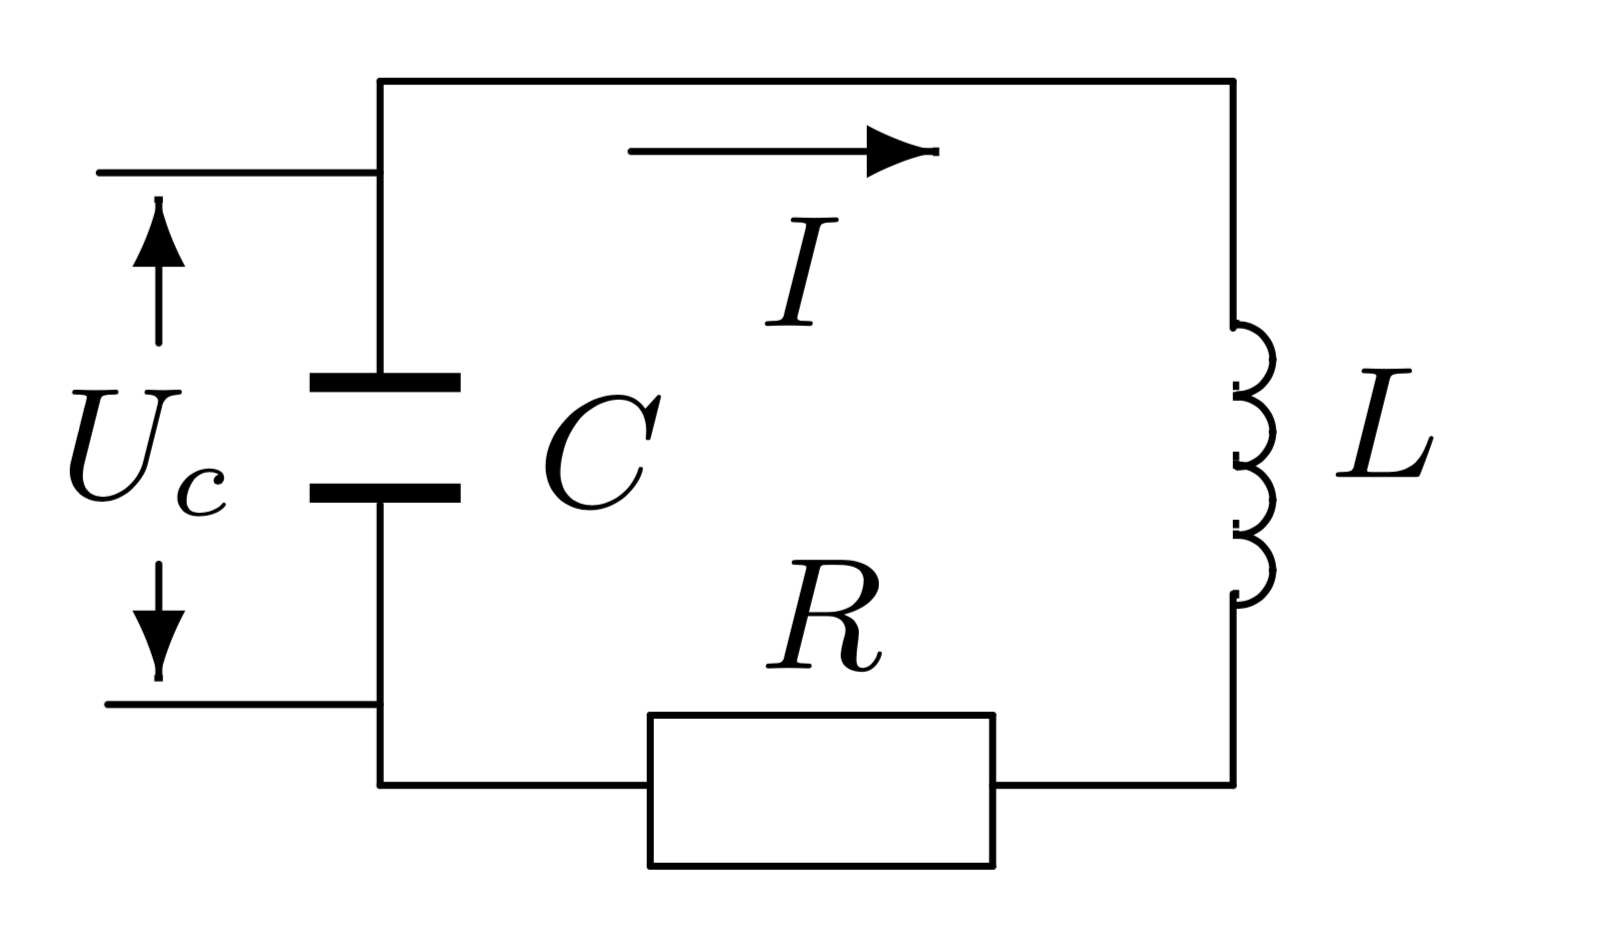
\includegraphics[width=6cm]{RLC}
	\caption{Колебательный контур}
	\label{RLC}
\end{wrapfigure}

Основное уравнение колебательного контура 

\begin{equation}\label{ddot I}
\ddot{I} + 2\gamma\dot{I} + \omega_0^2I = 0
\end{equation}

Где $ \gamma = \dfrac{R}{2L} $ --- коэффициент затухания, $ \omega_0^2 = \dfrac{1}{LC} $ --- собственная частота контура. Решением этого уравнения являются затухающие колебания:

\begin{equation}\label{}
I = A e^{-\gamma t} \cos (\omega t - \theta)
\end{equation}

Здесь $ \omega = \sqrt{\omega_0^2 - \gamma^2} $. Можно записать решение \eqref{ddot I} и для напряжения:

\begin{equation}\label{}
U_C = U_0 \dfrac{\omega_0}{\omega} e^{-\gamma t}\cos (\omega t - \theta)
\end{equation}

В контуре со слабым затуханием $ (\omega \backsimeq \omega_0) $ верна \textbf{формула Томпсона} для периода: 

\begin{equation}\label{}
T = \dfrac{2\pi}{\omega_0} \backsimeq  \dfrac{2\pi}{\omega} = 2\pi\sqrt{LC}
\end{equation}

Режим работы контура, при котором $ \gamma = \omega_0 $, называется \textbf{критическим}. Его сопротивление равно 

\begin{equation}\label{}
R_{кр} = 2\sqrt{\dfrac{L}{C}}
\end{equation}

Потери затухающих колебаний принято характеризовать через \textbf{добротность} и \textbf{логарифмический декремент затухания}: 

\begin{equation}\label{Q}
Q = 2\pi \dfrac{W}{\Delta W} = \dfrac{1}{R} \sqrt{\dfrac{L}{C}} \quad - \quad \text{Добротность, потери энергии}
\end{equation}
\begin{equation}\label{theta}
\Theta = \dfrac{1}{n} \gamma T = \dfrac{1}{n} \ln \dfrac{U_k}{U_{k+n}}  \quad - \quad \text{Лог. декремент, потери амплитуды}
\end{equation}

\section{Экспериментальная установка}
Исследуемый колебательный контур состоит из индуктивности $ L $,
ёмкости $ С $ и резистора $ R $ (рис. \ref{RLC}). Конденсатор контура заряжается
короткими одиночными импульсами, после каждого из которых в контуре
возникают свободные затухающие колебания. Подав напряжение
с конденсатора на осциллограф, можно по картине, возникающей на
экране осциллографа, определить период колебаний в контуре, исследовать
затухание колебаний и определить основные параметры колебательного
контура.

Картину колебаний можно представить не только в координатах ($ U, t $), но и в координатах ($ U, \dot{U} $), или, как говорят, на фазовой
плоскости. В этих координатах кривая незатухающих колебаний ( $ \gamma = 0 $)
имеет вид эллипса (или окружности - при одинаковых амплитудах $ U $
и $ \dot{U} $), а картина реальных колебаний изображается сворачивающейся
спиралью. 


\begin{wrapfigure}{r}{0.35\linewidth} 
	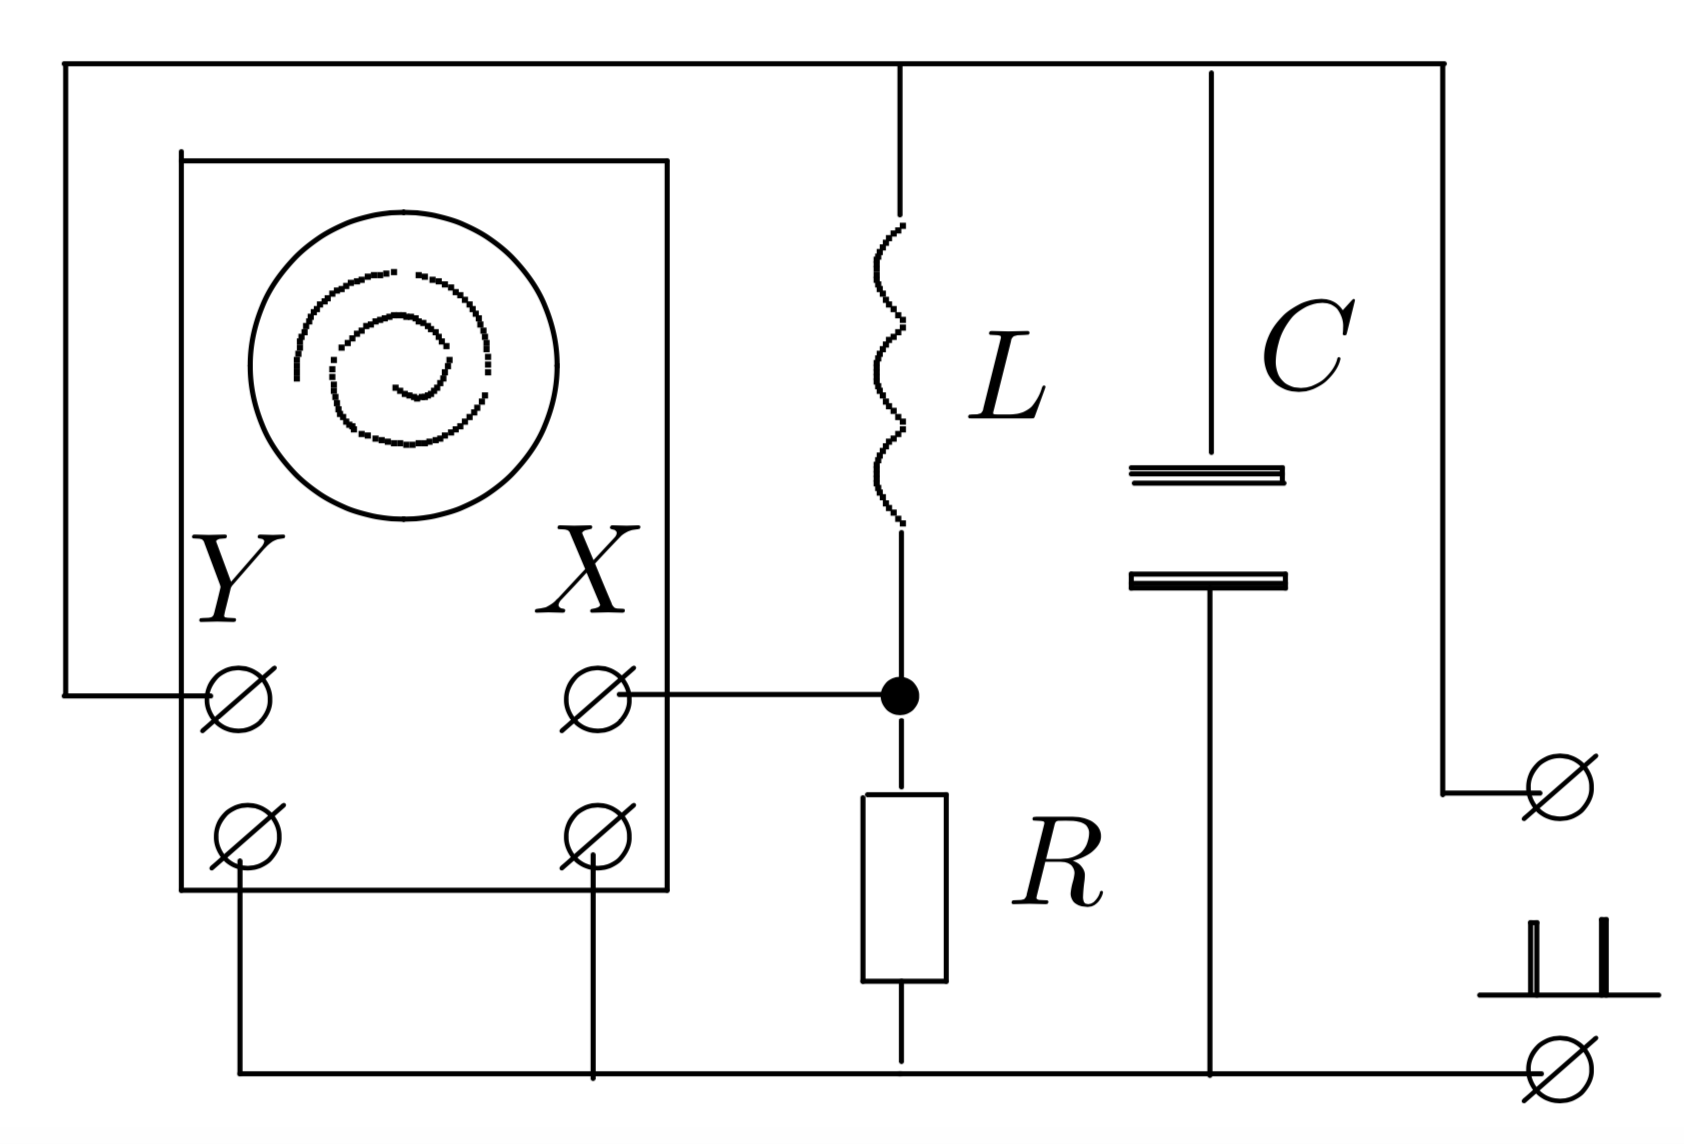
\includegraphics[width=6cm]{Fase}
	\caption{Фазовый режим}
	\label{Fase}
\end{wrapfigure}

Схема подключения осциллографа для изучения колебаний на фазовой плоскости представлена на рис. \ref{Fase}. На вертикальный вход осциллографа подаётся напряжение $ U_C $ с конденсатора, а на горизонтальный --- напряжение с резистора $ U_R $.

На рис. \ref{lab} приведена схема для исследования свободных колебаний в контуре типа рис. \ref{RLC}. Колебания наблюдаются на экране осциллографа.

Для периодического возбуждения колебаний в контуре используется
генератор импульсов Г5-54. С выхода генератора по коаксиальному кабелю импульсы поступают на колебательный контур через электронное
реле, смонтированное в отдельном блоке ( или на выходе генератора).
Реле содержит диодный тиристор1 $ D $ и ограничительный резистор $ R_1 $.
Импульсы заряжают конденсатор $ С $. После каждого импульса генератор
отключается от колебательного контура, и в контуре возникают
свободные затухающие колебания. Входное сопротивление осциллографа
велико ($ \backsimeq 1$ МОм), так что его влиянием иа контур можно пренебречь.

\begin{figure}[h]
	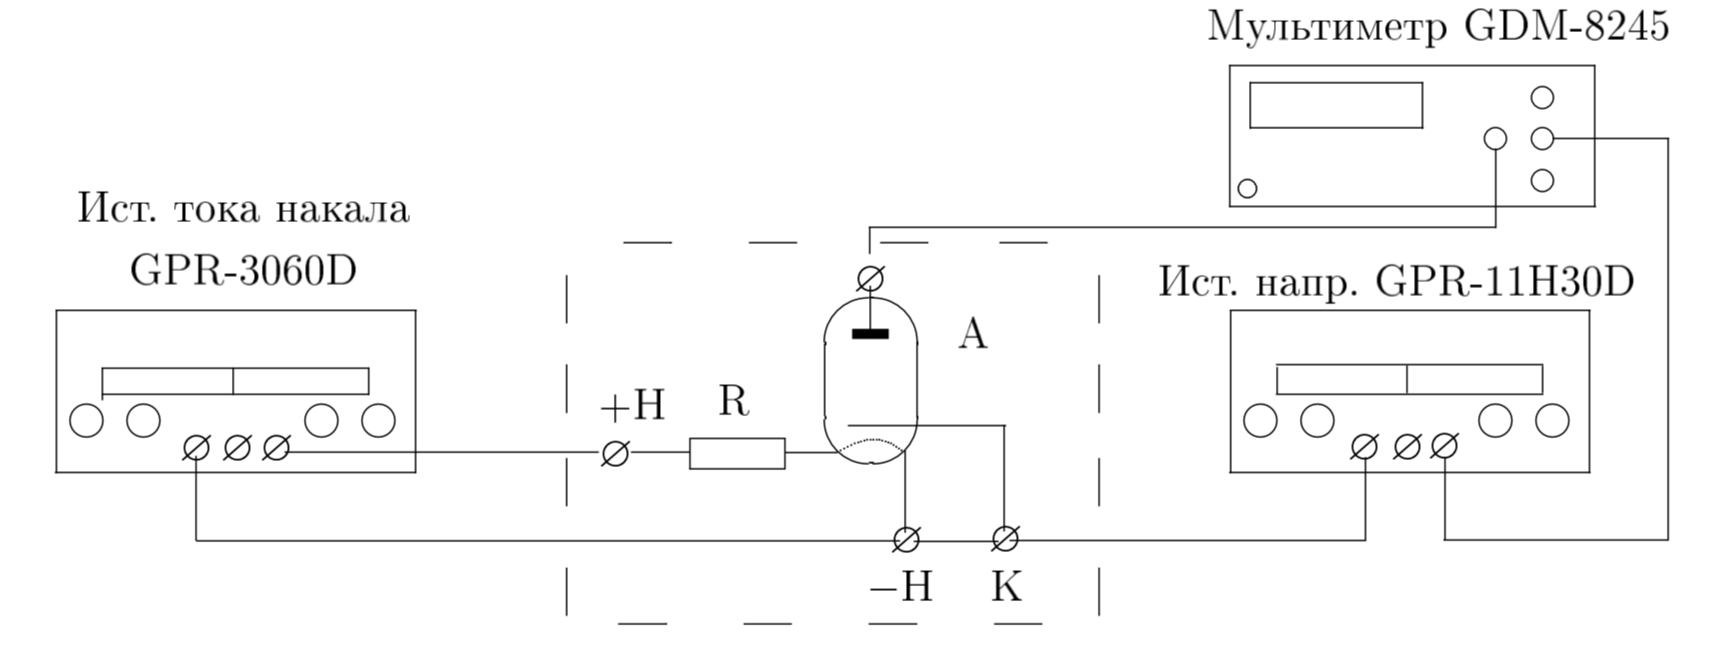
\includegraphics[width=15cm]{lab}
	\caption{Схема экспериментальной установки}
	\label{lab}
\end{figure}

Для получения устойчивой картины затухающих колебаний используется
режим ждущей развёртки с синхронизацией внешними импульсами,
поступающими с выхода "<синхроимпульсы"> генератора.

\section{Ход работы}

\subsection{Измерение периодов}

Проведем измерения при $ R = 0 $. Будем изменять емкость от $ 0,02 $ до 90 мкФ, проводя измерения периода по формуле:

\begin{equation}\label{}
T_{эксп} = T_0 \dfrac{x}{nx_0}
\end{equation}

где $ T_0 = 0,01 $ c, $ x_0 $ --- расстояние одного импульса, $ x $ --- расстояние $ n $ импульсов. Погрешность $ \sigma_x = \sigma_{x_0} = 0,1, \sigma_{T_0} = 0,001  $c. Тогда 

\begin{equation}\label{}
\sigma_{T_э} = T_э \sqrt{ \left( \dfrac{ \sigma_x}{x} \right)^2 + \left( \dfrac{ \sigma_{x_0}}{x_0} \right)^2  +  \left( \dfrac{ \sigma_{T_0}}{T_0} \right)^2}
\end{equation}

А $ T_{теор} = 2\pi\sqrt{LC} $, где $ L = 393 $ мГн, $ \sigma_L = 7 $ мГн (получено как среднее и среднее отклонение от рассчитанных $ L = 383, 386, 393, 400 $). $ \dfrac{\sigma_C}{C} \approx 0 $. Тогда 

\begin{equation}\label{}
\sigma_{T_т} = \dfrac{1}{2} \dfrac{\sigma_L}{L}
\end{equation}

Результаты сведем в таблицу \ref{resT} и построим график рис. 4. 

\begin{table}[h!]
	\centering
	\caption{Результаты измерений}
	\begin{tabular}{|c|c|c|c|c|c|c|c|}
		\hline
		$ С,$ мкФ & $ x_0 $ & $ n $ & $ x $ & $ T_{эксп}, мс $& $ \sigma_{T_э} $, мс & $ T_{теор}, мс $ & $ \sigma_{T_т} $, мс \\
		\hline
		0.02 & 6.0 & 2 & 0.7 & 0.58 & 0.2 & 0.56 & 0.01 \\
		0.09 & 3.0 & 2 & 0.6 & 1.00 & 0.39 & 1.18 & 0.02 \\
		0.15 & 6.0 & 4 & 3.5 & 1.46 & 0.17 & 1.52 & 0.02 \\
		0.22 & 6.0 & 3 & 3.0 & 1.67 & 0.21 & 1.84 & 0.02 \\
		0.35 & 6.0 & 3 & 3.3 & 1.83 & 0.22 & 2.32 & 0.03 \\
		0.48 & 6.0 & 3 & 4.0 & 2.22 & 0.26 & 2.72 & 0.04 \\
		0.59 & 6.5 & 3 & 4.5 & 2.31 & 0.26 & 3.02 & 0.04 \\
		0.75 & 6.5 & 2 & 3.4 & 2.62 & 0.32 & 3.4 & 0.04 \\
		0.87 & 6.5 & 2 & 4.3 & 3.31 & 0.38 & 3.66 & 0.05 \\
		0.90 & 6.5 & 2 & 4.6 & 3.54 & 0.4 & 3.72 & 0.05 \\
		\hline
	\end{tabular}% 
\label{resT}% 
\end{table}% 

\begin{figure}[h!]
	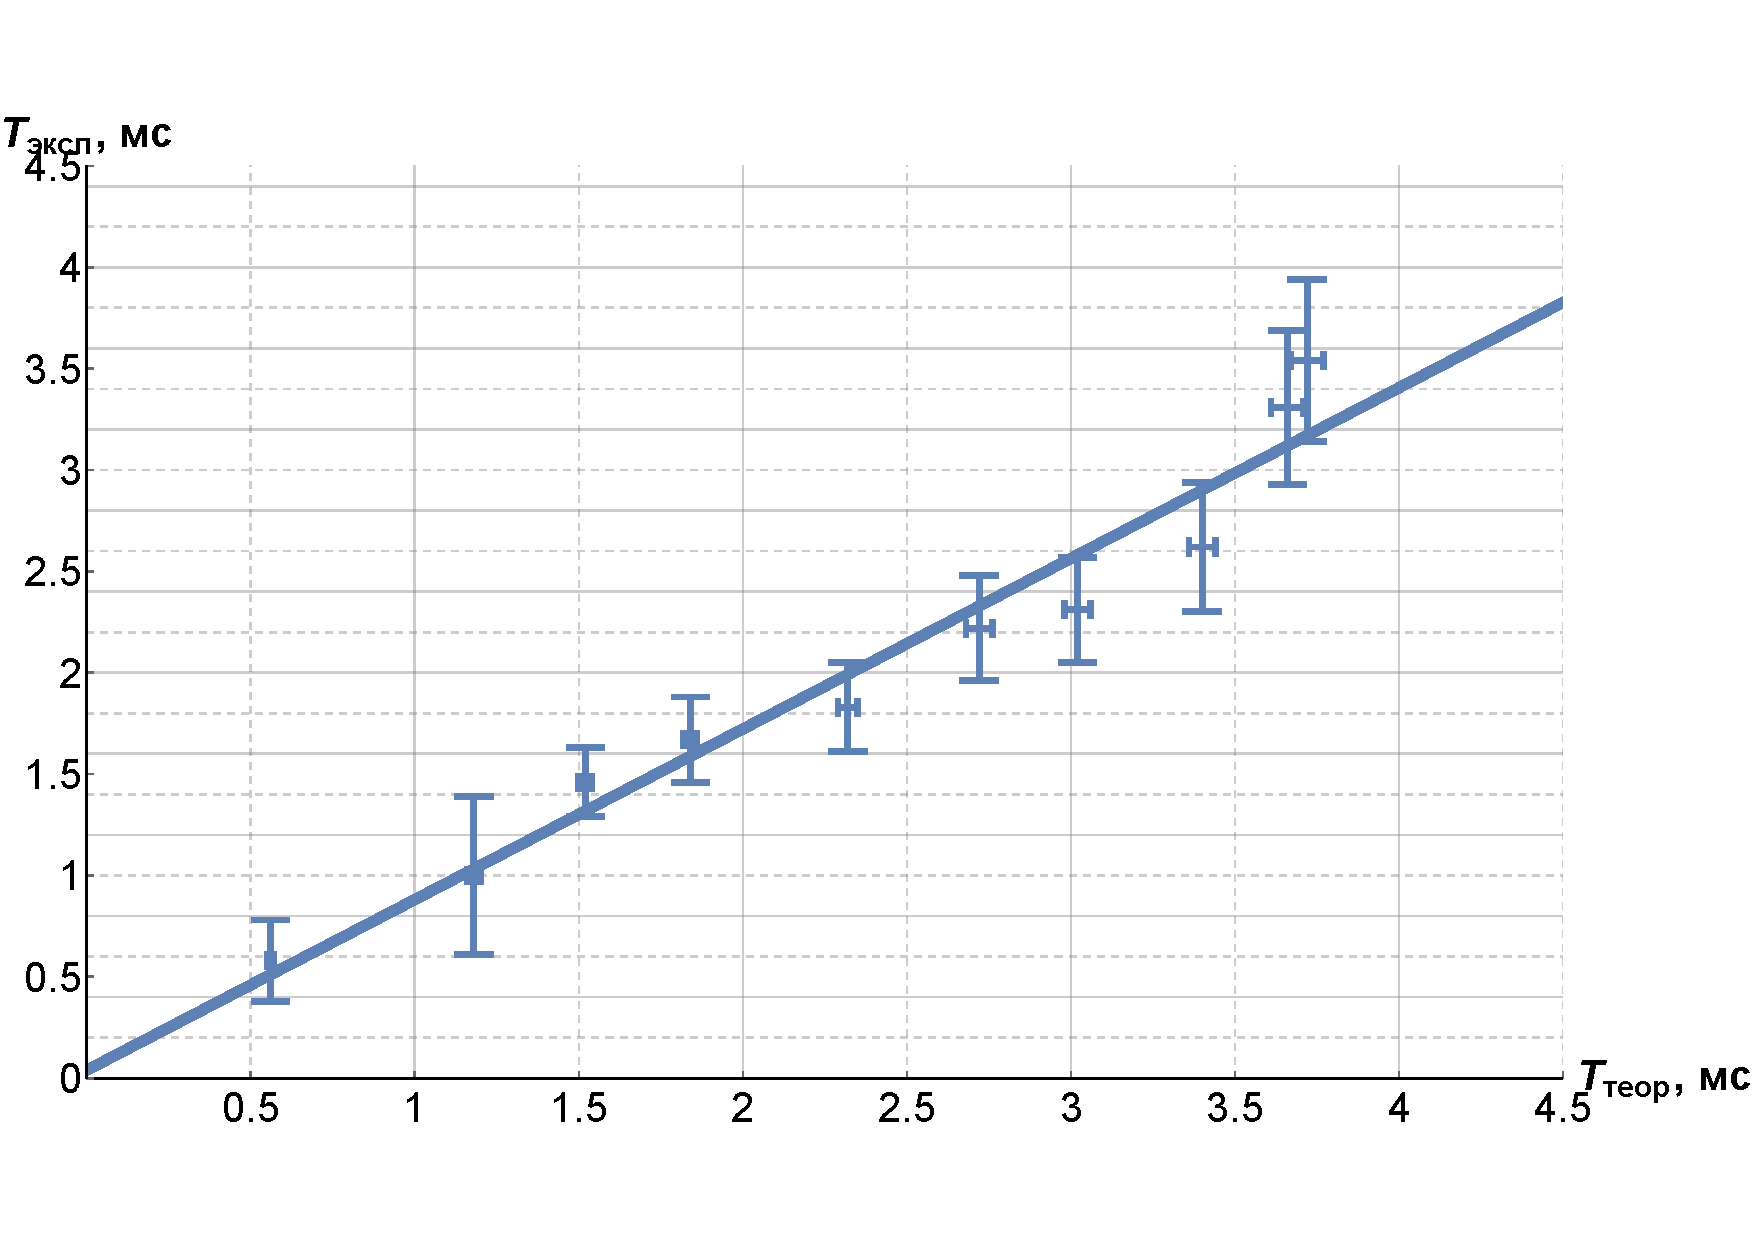
\includegraphics[scale=0.55]{T.pdf}
	\caption{Зависимость $ T_{теор}$ от $ T_{эксп} $}
\end{figure}

\subsection{Критическое сопротивление и декремент затухания}

Теперь, считая $ L = 200 $ мГн, вычислим  частоту емкость, считая $ \nu_0 = \dfrac{1}{LC} = 5 $ кГц $ \te C = 5  $ нФ. Тогда 
 
 \begin{equation}\label{}
 R_ {кр} = 2 \sqrt{\dfrac{L}{C}} \approx 12,6 кОм
 \end{equation}

Установим эту $ С $ на магазине емкостей, будем наблюдать картину затухающих колебаний, изменяя $ R $ от $ 0,1 R_{кр}$ до $ R_{кр} $. Сопротивление магазина, при котором колебания переходят в апериодический, примерно равен критическому. 

\begin{table}[h!]
	\centering
	\caption{Результаты измерений}
	\begin{tabular}{|c|c|c|c|c|c|c|c|}
		\hline
		$ R $, Ом & $ n $ & $ U_k$ & $ U_{k+n} $& $ \Theta $& $ \sigma_\Theta $ & $ R_к $, Ом & $ \sigma_{R_к} $, Ом \\
		\hline
		1100 & 3 & 3.0 & 0.9 & 0.40 & 0.05 & 1142 & 2 \\
		1400 & 3 & 3.0 & 0.6 & 0.54 & 0.09 & 1442 & 3 \\
		1800 & 2 & 2.9 & 0.8 & 0.64 & 0.08 & 1842 & 4 \\
		2200 & 2 & 2.8 & 0.6 & 0.77 & 0.13 & 2242 & 4 \\
		2500 & 1 & 2.7 & 1.0 & 0.99 & 0.11 & 2542 & 5 \\
		2700 & 1 & 2.6 & 0.9 & 1.06 & 0.12 & 2742 & 5 \\
		3300 & 1 & 2.5 & 0.8 & 1.14 & 0.15 & 3342 & 7 \\
		3600 & 1 & 2.5 & 0.7 & 1.27 & 0.19 & 3642 & 7 \\
		\hline
	\end{tabular}% 
	\label{resR}% 
\end{table}% 

Теперь, изменяя сопротивление от примерно $ 0,1 R_{кр} $ до $ 0,3 R_{кр} $, будем измерять амплитуды колебаний, разделенных на $ n $ частей, для вычисления декремента по формуле \eqref{theta}. Погрешности амплитуд $  \sigma_{U_k} = \sigma_{U_{k+n}} = 0,1 $, т.е. 

\begin{equation}\label{}
\sigma_{\Theta} = \Theta \sqrt{ \left( \dfrac{ \sigma_{U_k}}{U_k} \right)^2 + \left( \dfrac{ \sigma_{U_{k+n}} }{U_{k+n}} \right)^2 }
\end{equation}

Измерив на универсальном мосте сопротивление катушки при нашей частоте 5 кГц, добавим его к сопротивлению магазина, получив сопротивление контура$ R_к $. Результаты сведем в таблицу \ref{resR}. Теперь построим график $ \dfrac{1}{\Theta^2} $ от $ \dfrac{1}{R^2} $, считая погрешность $ \sigma_{\frac{1}{\Theta^2}} = 2 \dfrac{1}{\Theta^2} \dfrac{\sigma_\Theta}{\Theta}$ Данные для графика  рис. 5 сведены в таблице \ref{res}.



\begin{table}[h!]
	\centering
	\caption{Результаты измерений}
	\begin{tabular}{|c|c|c|}
		\hline
	$ \dfrac{1}{\Theta^2} $& $ \sigma_{\frac{1}{\Theta^2}} $ & $ \dfrac{1}{R^2}, 10^{-6} Ом^{-2}$  \\
		\hline
		6.21 & 0.75 & 0.77 \\
		3.47 & 0.68 & 0.48 \\
		2.41 & 0.63 & 0.29 \\
		1.69 & 0.57 & 0.2 \\
		1.01 & 0.22 & 0.15 \\
		0.89 & 0.21 & 0.13 \\
		0.77 & 0.2 & 0.09 \\
		0.62 & 0.18 & 0.08 \\
		\hline
	\end{tabular}% 
	\label{res}% 
\end{table}% 

\begin{figure}[h!]
	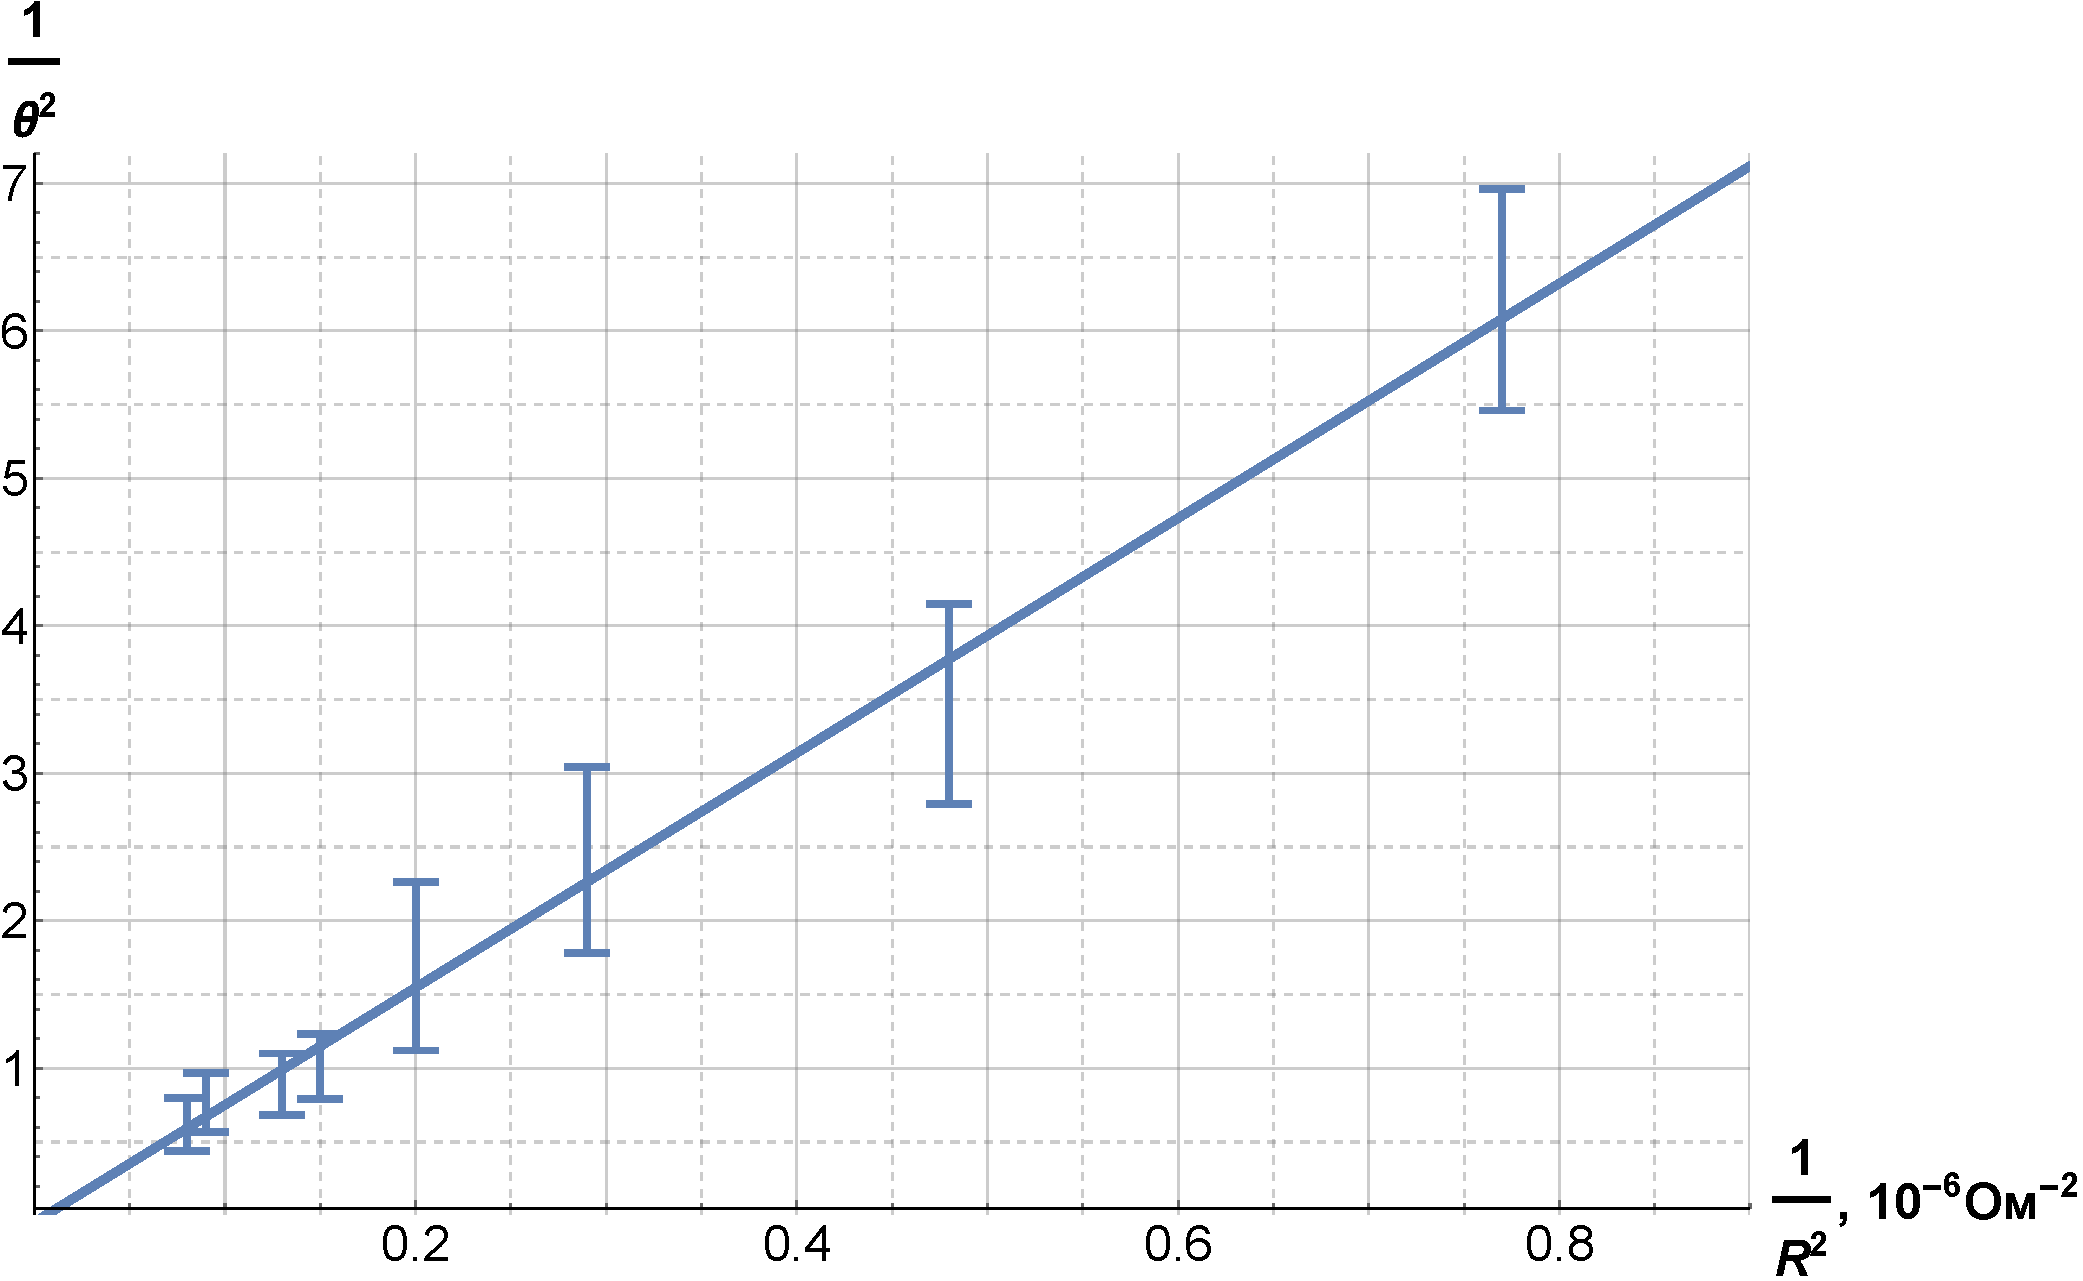
\includegraphics[scale=0.5]{teta.pdf}
	\caption{Зависимость $ \dfrac{1}{\Theta^2} $ от $ \dfrac{1}{R^2} $}
\end{figure}

Аппроксимируя полученные данные, получаем следующий результат: 

\begin{table}[h!]%{l}{0.5\linewidth}
	\centering
	\caption{Расчет апроксимированной прямой $ y = ax +b $}
	\begin{tabular}{c|cc}
		\text{} & \text{Estimate} & \text{Standard Error} \\
		\hline
		b & 0.039 & 0.176  \\
		a & 7.957 & 0.281  \\
	\end{tabular}
\end{table}

Если заменить $ \dfrac{1}{\Theta^2} = Y $, $ \dfrac{1}{R^2} = X $, то получаем, что $ \dfrac{\Delta Y}{\Delta X} = 7.957 \x 10^6 \; Ом^2$. Посчитаем 

\begin{equation}\label{}
R_{кр} = 2\pi \sqrt{\dfrac{\Delta Y}{\Delta X} } \approx 17,71 \; кОм
\end{equation}

Погрешность равна $ \sigma_{R_{кр}} = R_{кр} \dfrac{1}{2} \dfrac{\sigma_a}{a} \approx 0,31 $ кОм. 

Вычислим теоретическое значение $ R_{кр}  = 2\sqrt{\dfrac{L}{C}}$, где $ C = 5 $ нФ, $ L = 393 $ мГн. Получаем $ R_{кр} \approx 17,73 $ кОм, погрешность $ \sigma_{R_{кр}} = R_{кр} \dfrac{1}{2} \dfrac{\sigma_L}{L} \approx 0,33 $ кОм. 

Таким образом, мы видим, что эти результаты прекрасно согласуются между собой. 

\subsection{Добротность}

По формуле \eqref{Q} посчитаем добротность через параметры контура $ C = 5 $ нФ, $ L = 393 $ мГн, беря минимум и максимум сопротивления контура из таблицы \ref{resR}. Погрешность равна $ \sigma_Q = Q \dfrac{1}{2} \dfrac{\sigma_L}{L} $.

\begin{equation}\label{}
R = 1,1 \; кОм, \qquad Q = 7,76 \pm 0,09
\end{equation}
\begin{equation}\label{}
R = 3,6 \; кОм, \qquad Q = 2,43 \pm 0,03
\end{equation}

Теперь сделаем это по формуле 

\begin{equation}\label{}
Q = \dfrac{\pi}{\Theta}
\end{equation}

Аналогично возьмем минимум и максимум декремента из таблицы \ref{resR}. Погрешность равна $ \sigma_Q = Q \dfrac{\sigma_\Theta}{\Theta} $. 

\begin{equation}\label{}
\Theta = 0,4 ,\qquad Q = 7,82 \pm 0,51
\end{equation}
\begin{equation}\label{}
\Theta = 1,27 ,\qquad Q = 2,47 \pm 0,27
\end{equation}

Теперь возьмём логарифмический декремент затухания, полученные через отношения радиусов спиралей, т.е. $ \Theta =  \dfrac{1}{n} \ln \dfrac{r_k}{r_{k+n}}$. Радиус мы будем измерять, наблюдая картину фазовых колебаний (см. рис. \ref{Fase}). При $ R = 1,2  $ кОм, $ r_k = 0,7, r_{k+3} = 3,1 \te \Theta \approx 0,51. $ При $ R = 3,6  $ кОм, $ r_k = 0,6, r_{k+1} = 2,4 \te \Theta \approx 1,39.$ Погрешность считается аналогично формулам выше. Получаем:

\begin{equation}\label{}
\Theta = 0,51 ,\qquad Q = 6,33 \pm 0,87
\end{equation}
\begin{equation}\label{}
\Theta = 1,27 ,\qquad Q = 2,27 \pm 0,43
\end{equation}


\section{Вывод}

Итак, в этой работе мы изучили свободные колебания в электрическом контуре: сначала измеряли периоды при $ \gamma \approx 0 $, затем находили критическое сопротивление и изучали колебательный контур при сопротивлениях порядка $ 0,1 -- 0,4 R_{кр} $. Мы исследовали зависимость логарифмического декремента затухания от сопротивления контура, а также добротности от параметров контура и от декремента. 

Основные результаты занесены в таблицы:
\begin{table}[h!]%{l}{0.5\linewidth}
	\centering
	\caption{Расчет критического сопротивления }
	\begin{tabular}{|c|c|c|c|}
		\hline
		\multirow{2}{*}{$  L $} & \multicolumn{3}{|c|}{$ R_{кр} $} \\
		\cline{2-4}
		& Теор. & Подбор & Граф.  \\
		\hline
		$ 393 \pm  7 $ мГн   & $ 17,73 \pm 0,33 $ кОм & 12,6 кОм & 	$ 17,71 \pm 0,31 $ кОм \\
		\hline
	\end{tabular}
\end{table}

\begin{table}[h!]%{l}{0.5\linewidth}
	\centering
	\caption{Расчет добротности}
	\begin{tabular}{|c|c|c|c|}
		\hline
		\multirow{2}{*}{$ R $} & \multicolumn{3}{|c|}{$ Q $} \\
		\cline{2-4}
		& Теор. & $ f(\Theta) $ & Спираль \\
		\hline
		1242 Ом & $ 7,76 \pm 0,09 $ & $ 7,82 \pm 0,51 $ & $ 6,33 \pm 0,87 $ \\
		\hline
		3642 Ом  & $ 2,43 \pm 0,03 $ & $ 2,47 \pm 0,27 $  & $ 2,27 \pm 0,43 $ \\
		\hline
	\end{tabular}
\end{table}




\end{document}